\documentclass{standalone}
\usepackage{tikz}
\begin{document}%
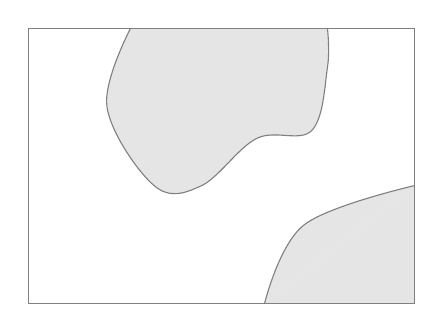
\begin{tikzpicture}[font=\small]

% obstacle 1 fill
\fill[black!10] plot [smooth,tension=0.6] coordinates {
   (1.3,3.5) (1.0,2.5) (1.6,1.5) (2.2,1.5)
   (2.9,2.1) (3.6,2.2) (3.8,3.0) (3.8,3.5)};

% obstacle 2 fill
\fill[black!10] plot [smooth,tension=0.6] coordinates {
   (3.0,0.0) (3.5,1.0) (4.9,1.5)};
\fill[black!10] (4.9,1.5) -- (4.9,0.0) -- (3.0,0.0) -- cycle;

% obstacle 1 boundary
\draw[black!50] plot [smooth,tension=0.6] coordinates {
   (1.3,3.5) (1.0,2.5) (1.6,1.5) (2.2,1.5)
   (2.9,2.1) (3.6,2.2) (3.8,3.0) (3.8,3.5)};

% obstacle 2 boundary
\draw[black!50] plot [smooth,tension=0.6] coordinates {
   (3.0,0.0) (3.5,1.0) (4.9,1.5)};

% obstacle labels
%\node[text=black!70] at (2.6,3.0) {$CO_1$};
%\node[text=black!70] at (4.1,0.6) {$CO_2$};

% path
%\draw plot [smooth,tension=0.6,thick] coordinates {
%   (0.5,2.0) (1.0,1.0) (2.8,1.0) (4.0,1.9) (4.4,2.2)};

% path endpoints / labels
%\fill[black] (0.5,2.0) circle (0.05cm);
%\fill[black] (4.4,2.2) circle (0.05cm);
%\node at (0.5,2.2) {$q_{\mbox{\tiny start}}$};
%\node at (4.4,2.4) {$q_{\mbox{\tiny goal}}$};

% C label
%\node[text=black,anchor=north west] at (0.0,3.5) {$\mathcal{C}$};

% C-space border
\draw[black!50] (0,0) rectangle (4.9,3.5);

% add a grid at 1cm resolution
%\draw[step=1cm,gray,very thin] (0,0) grid (5,4);

\end{tikzpicture}%
\end{document}
